\section{Фильтры}
\begin{center}
    Конспект составил: \textit{Арсений Кузнецов}
\end{center}

\subsection{Сглаживание}

\textbf{Сглаживание}~--- технология, которая позволяет справиться с эффектом ступенчатости, обусловленным дискретностью растра. Данный эффект проявляется при создании любой наклонной линии в растре. Пример сглаживания Рис.~\ref{fig:image1}-\ref{fig:image2}.

\begin{figure}[h!]
    \centering
    % Первое изображение
    \begin{minipage}{0.3\textwidth}
        
\includegraphics[width=\textwidth]{дуга.png} % Укажите путь к файлу
        \caption{Дуга без сглаживания}
        \label{fig:image1}
    \end{minipage} % Горизонтальный отступ между изображениями
    % Второе изображение
    \hspace{0.1\textwidth}
    \begin{minipage}{0.3\textwidth}
        
\includegraphics[width=\textwidth]{сглаженная дуга.png} % Укажите путь к файлу
        \caption{Дуга сглаженная методом полутонов}
        \label{fig:image2}
    \end{minipage}
\end{figure}

Методы сглаживания:
\begin{enumerate}
    \item измельчение растра
    \item метод полутонов
\end{enumerate}

\subsubsection{Измельчение растра}

\textbf{Измельчение растра}~--- масштабирование изображения путем увеличения количества пикселей в сетке.
При измельчении растра мы можем поставить новые ячейки в промежутках между старыми и посчитать значения новых ячеек на основании значения старых. Пример на Рис.~\ref{fig:rastr1}-\ref{fig:rastr2}.

\begin{figure}[h!]
    \centering
    % Первое изображение
    \begin{minipage}{0.3\textwidth}
        $$
            \begin{matrix}
                \bullet &  & \bullet &  & \bullet \\ \\ \bullet & & \bullet & & \bullet \\ \\ \bullet &  & \bullet & &  \bullet
            \end{matrix}
        $$
        \caption{Оригинальный растр}
        \label{fig:rastr1}
    \end{minipage} % Горизонтальный отступ между изображениями
    % Второе изображение
    \hspace{0.1\textwidth}
    \begin{minipage}{0.3\textwidth}
        $$
            \begin{matrix}
                \bullet & \circ & \bullet & \circ & \bullet \\
                \circ   & \circ & \circ   & \circ & \circ   \\
                \bullet & \circ & \bullet & \circ & \bullet \\
                \circ   & \circ & \circ   & \circ & \circ   \\
                \bullet & \circ & \bullet & \circ & \bullet
            \end{matrix}
        $$
        \caption{Измельченный растр}
        \label{fig:rastr2}
    \end{minipage}
\end{figure}

Как мы будем определять каким цветом закрасить новые ячейки?
Возьмем часть измельченного растра:
$$
    \begin{matrix}
        \circ & \circ   & \circ \\
        \circ & \bullet & \circ \\
        \circ & \circ   & \circ
    \end{matrix}
$$

И скажем, что первоначальная точка мажорирует с соседними со следующими параметрами:

$$
    \begin{matrix} 1 & 2 & 1 \\ 2 & \bf4 & 2 \\ 1& 2 & 1 \end{matrix}
$$

\begin{callout}{Пояснение}
    Изначальная точка останется с тем же цветом, что и была. Цвет точек по горизонтали и вертикали будет средним между двумя изначальными, а цвет точек на диагоналях~--- средним между четырьмя соседними точками.
\end{callout}

До этого мы добавляли одну точку между двумя изначальными. Теперь рассмотрим пример на Рис.~\ref{fig:rastr3}-\ref{fig:rastr4}, где мы добавляем 3 точки (рассмотрим только четверть квадрата).

\begin{figure}[h!]
    \centering
    % Первое изображение
    \begin{minipage}{0.3\textwidth}
        $$
            \begin{matrix}
                \circ & \circ & \circ & \circ   \\
                \circ & \circ & \circ & \circ   \\
                \circ & \circ & \circ & \circ   \\
                \circ & \circ & \circ & \bullet
            \end{matrix}
        $$
        \caption{Измельченный растр}
        \label{fig:rastr3}
    \end{minipage} % Горизонтальный отступ между изображениями
    % Второе изображение
    \hspace{0.1\textwidth}
    \begin{minipage}{0.3\textwidth}
        $$
            \begin{matrix}
                1 & 2 & 3  & 4       \\
                2 & 4 & 6  & 8       \\
                3 & 6 & 9  & 12      \\
                4 & 8 & 12 & \bf{16}
            \end{matrix}
        $$
        \caption{Параметры измельченного растра}
        \label{fig:rastr4}
    \end{minipage}
\end{figure}

Отсюда видно, что каждый изначальный пиксель оказывает влияние не только на соседей, но и на все пиксели вплоть до следующего.

\subsection{Яркость}

\textbf{Яркость}~--- отличие изображение от черного. Более точно определяется как мат ожидание насыщенности по R, G, B.

$$Br = {\underset{\text{colour} \in \text{pixel}}{\mathsf{E}} \text{colour}}$$

\begin{callout}{Примечание}
    В нашем случае, мат ожидание вырождается в среднее арифметическое по цветам.
\end{callout}

Изобразим набор значений, для которых яркость равна константе~\ref{fig:constbr}\footnote{На примерах будет использоваться только два цвета из стандартных трех, чтобы изображать на плоскости, а не в пространстве.}.

\begin{figure}[h!]
    \centering
    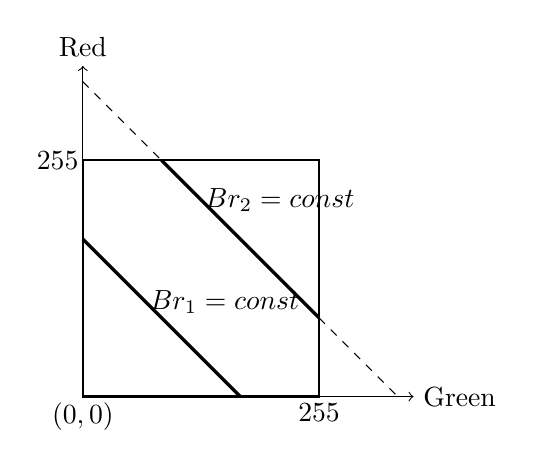
\begin{tikzpicture}
        % Draw the outer square
        \draw[thick] (0,0) rectangle (3,3);

        % Draw coordinate axes
        \draw[->] (0, 0) -- (4.2,0) node[right] {Green}; % X-axis
        \draw[->] (0,0) -- (0,4.2) node[above] {Red}; % Y-axis
        \node at (0,-0.25) {$(0, 0)$};
        \node at (3,-0.2) {$255$};
        \node at (-0.32, 3) {$255$};

        % Draw lines and annotations inside the upper right quadrant
        \draw[very thick] (0,2) -- (2,0); % Diagonal line
        \node at (1.8,1.2) {$Br_1 = const$};
        \draw[dashed] (0, 4) -- (1, 3);
        \draw[very thick] (1,3) -- (3,1); % Diagonal line
        \draw[dashed] (3,1) -- (4, 0);
        \node at (2.5,2.5) {$Br_2 = const$};
    \end{tikzpicture}
    \caption{Множество цветов с константной яркостью}
    \label{fig:constbr}
\end{figure}

Так как 255 максимальное значение для каждого цвета, следовательно, выйти за пределы выше изображенного квадрата мы не можем. Поэтому, в случае трех цветов, максимальной яркостью будет обладать одна точка $(255, 255, 255)$~--- белый цвет.

\subsubsection{Увеличение яркости}

Хотим увеличить яркость в точке $(x, y)$ в $n$ раз.
Для этого:
\begin{enumerate}
    \item Умножим $x$, $y$ на $n$, получим $(x*n, y*n)$.
    \item Если точка лежит не в квадрате, то проведем прямую из $(0, 0)$ в полученную точку и найдем пересечение прямой с квадратом. Точка пересечения и будет результатом\footnote{Данный шаг нужен, чтобы не выйти за границы доступных цветов и при этом сохранить изначальное соотношение цветов.}.
\end{enumerate}
Пример на Рис.~\ref{fig:upbr}.

\begin{figure}[h!]
    \centering
    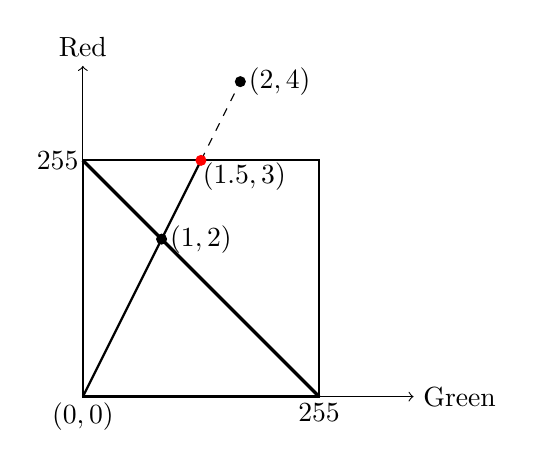
\begin{tikzpicture}
        % Draw the outer square
        \draw[thick] (0,0) rectangle (3,3);

        % Draw coordinate axes
        \draw[->] (0, 0) -- (4.2,0) node[right] {Green}; % X-axis
        \draw[->] (0,0) -- (0,4.2) node[above] {Red}; % Y-axis
        \node at (0,-0.25) {$(0, 0)$};
        \node at (3,-0.2) {$255$};
        \node at (-0.32, 3) {$255$};

        % Draw lines and annotations inside the upper right quadrant
        \draw[very thick] (0,3) -- (3,0); % Diagonal line
        \fill (1,2) circle (2pt); % Точка радиусом 2pt
        \node at (1.5, 2) {$(1, 2)$};
        \node at (2.05, 2.8) {$(1.5, 3)$};
        \draw[thick] (0, 0) -- (1.5, 3);
        \draw[dashed] (1.5, 3) -- (2, 4);
        \fill[color=red](1.5, 3) circle (2pt);
        \fill (2, 4) circle (2pt);
        \node at (2.5, 4) {$(2, 4)$};
    \end{tikzpicture}
    \caption{Увеличение яркости в точке $(1, 2)$ в 2 раза, с результатом $(1.5, 3)$}
    \label{fig:upbr}
\end{figure}

\begin{callout}{Замечание}
    Отсюда можно увидеть, что при последующем уменьшении яркости, можно получить более темное изображение, чем оно было изначально.

    Пример:
    $(1.5, 3)/2 = (0.75, 1.5)$, хотя исходная точка была $(1, 2)$
\end{callout}

\subsection{Контрастность}

\textbf{Контрастность} показывает насколько разные цвета на изображении и определяется через абсолютный центральный момент
$$K = \mathsf{E}|color - Br|$$

\begin{callout}{Замечание}
    Для измерения контрастности может подойти и дисперсия по цветам, если изменяем квадратично.
    $$\mathsf{D} \ color = \mathsf{E}|color - Br|^2$$
\end{callout}

Увеличение контрастности на $\alpha$~--- это домножение на $\alpha$ в комплексной плоскости (поворот на угол $\alpha$) \ref{fig:kontr}. Диагональ квадрата (серые цвета) имеет минимальную контрастность, а отклонение на угол от диагонали в любую сторону будет контрастность увеличивать.

\begin{figure}[h!]
    \centering
    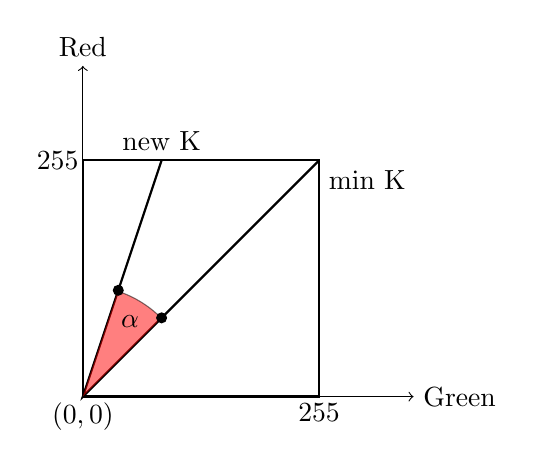
\begin{tikzpicture}
        % Draw the outer square
        \draw[thick] (0,0) rectangle (3,3);

        % Draw coordinate axes
        \draw[->] (0, 0) -- (4.2,0) node[right] {Green}; % X-axis
        \draw[->] (0,0) -- (0,4.2) node[above] {Red}; % Y-axis
        \node at (0,-0.25) {$(0, 0)$};
        \node at (3,-0.2) {$255$};
        \node at (-0.32, 3) {$255$};

        \coordinate[] (A) at (0,0);
        \coordinate[label=below right:min K] (X) at (3,3);
        \coordinate[label=above:new K] (Y) at (1, 3);

        \draw[thick] (X) -- (A) -- (Y);

        % Mark the angle XAY
        \begin{scope}
            \path[clip] (A) -- (X) -- (Y);
            \fill[red, opacity=0.5, draw=black] (A) circle (1.41);
        \end{scope}
        \node at (0.6, 0.95) {$\alpha$};
        \fill (1, 1) circle (2pt);
        \fill (0.45, 1.35) circle (2pt);
    \end{tikzpicture}
    \caption{Изменение контрастности на $\alpha$}
    \label{fig:kontr}
\end{figure}

\begin{callout}{Замечание}
    Порядок изменения яркости и контрастности важен!
    Так как из-за насыщения у нас есть ряд точек, в которых изменения неоднозначны.
\end{callout}

\subsubsection{Как делать быстро}

В полярных координатах считать долго, намного быстрее домножить на матрицу поворота, где поворот рассматривается относительно прямой серого.

\subsection{Повороты}
Заключается в повороте каждой точки изначального растра на градус. Для повернутых точек применяем аналог алгоритма Брезенхэма, который определяет какие пиксели надо закрасить явно, а какие в полутона.

\subsection{Фильтры}
\textbf{Фильтры} осуществляют некоторое преобразование над изображением, в ходе которого обычно создается новое изображение возможно даже другого размера. Преобразования обычно применяются к небольшому куску изображения, для применения ко всему изображению, используется свертка.

Размер окна преобразования определяет параметр фильтра. Размеры итогового и изначального окна могут совпадать, а могут не совпадать. Результаты преобразований окон могут также накладываться друг на друга в результирующем изображении.

Отдельная проблема при использовании фильтров~--- это обработка граничных пикселей. Для них существуют следующие варианты:
\begin{enumerate}
    \item не обрабатывать граничные значения;
    \item перераспределить веса по соседям;
    \item доопределить значения пикселей;
    \item зеркализация;
    \item замыкание на другую сторону.
\end{enumerate}

\subsubsection{Пример сглаживающего фильтра}

Возьмем окно $(2r+1)\times(2r+1)$ и заполним равномерно по формуле $\dfrac 1 {(2r+1)^2}$. Пусть $r = 1$, тогда получаем следующее окно влияния цвета пикселя на соседние:
$$
    \begin{matrix}
        \frac 1 9 & \frac 1 9 & \frac 1 9 \\
        \frac 1 9 & \frac 1 9 & \frac 1 9 \\
        \frac 1 9 & \frac 1 9 & \frac 1 9 \\
    \end{matrix}
$$

Значения за границами будем считать нулями. На Рис.~\ref{fig:filter1}-\ref{fig:filter2} приведен пример обработки фильтром на одноцветном изображении $4 \times 4$.

\begin{figure}[h!]
    \centering
    % Первое изображение
    \begin{minipage}{0.3\textwidth}
        $$
            \begin{matrix}
                9 & 0 & 0 & 0 \\
                0 & 9 & 0 & 0 \\
                0 & 0 & 9 & 0 \\
                0 & 0 & 0 & 0
            \end{matrix}
        $$
        \caption{Изображение до обработки сглаживающим фильтром}
        \label{fig:filter1}
    \end{minipage} % Горизонтальный отступ между изображениями
    % Второе изображение
    \hspace{0.1\textwidth}
    \begin{minipage}{0.3\textwidth}
        $$
            \begin{matrix}
                2 & 2 & 1 & 0 \\
                2 & 3 & 2 & 1 \\
                1 & 2 & 2 & 1 \\
                0 & 1 & 1 & 1
            \end{matrix}
        $$
        \caption{Изображение после обработки}
        \label{fig:filter2}
    \end{minipage}
\end{figure}
